\documentclass[a4paper, 11pt]{article}

%-------------------------------------------------------------------------------
%--- (a) Required Packages
%-------------------------------------------------------------------------------
\usepackage{amsmath,amsfonts,amssymb,amsthm}
\usepackage{adjustbox}
\usepackage{mwe}
\usepackage{authblk}
\usepackage[english]{babel}
\usepackage[para,online,flushleft]{threeparttable}
\usepackage{lscape}
\usepackage{threeparttablex}
\usepackage{tabu}
\usepackage{bm}
\usepackage{booktabs}
\usepackage{caption}
\usepackage{subcaption}
\usepackage[usenames, dvipsnames]{color}
\usepackage{epstopdf}
\usepackage[capposition=top]{floatrow}
\usepackage{framed}
%\usepackage[T1]{fontenc}
\usepackage{lmodern}
\usepackage{graphicx}
\usepackage{hyperref}
\usepackage[utf8]{inputenc}
\usepackage{lscape}
\usepackage{multirow}
\usepackage{natbib}
\usepackage{setspace}
\usepackage{rotating}
\usepackage{subcaption}
\usepackage{subfloat}
\usepackage{url}
\usepackage{wrapfig}
\usepackage{multicol}
\usepackage[toc,page]{appendix}
\usepackage{float}
\interfootnotelinepenalty=10000
\usepackage[margin=1in]{geometry}
\usepackage{textcomp}
\usepackage{longtable}
\usepackage{babel,blindtext}

%-------------------------------------------------------------------------------
%--- (b) Specific margins
%-------------------------------------------------------------------------------
%\setlength  \textwidth{\paperwidth}
%\setlength  \textheight{\paperheight}
%\setlength  \oddsidemargin{3cm}
%\setlength  \topmargin{-1.2cm}
%\setlength  \footnotesep{2ex}
%\addtolength\textheight{-6cm}
%\addtolength\textwidth{-6cm}
%\addtolength\oddsidemargin{-1in}
\setlength\parskip{0.25in} 
 
%%ADDED SPACE BETWEEN PARAGRAPHS 
%-------------------------------------------------------------------------------
%--- (c) Internal Ref stype
%-------------------------------------------------------------------------------

\hypersetup{            
    colorlinks=true,   
    linkcolor=Black,
    citecolor=BlueViolet,
    filecolor=BlueViolet,
    urlcolor=Black
}

 
%-------------------------------------------------------------------------------
%--- (1) Title
%-------------------------------------------------------------------------------
\title{The Impact of Abortion Legalization on Fertility and Maternal Mortality: New Evidence from Mexico\thanks{We are grateful to Andreea Mitrut, Randi Hjalmarsson, Elin Larsson, Blair G. Darney, Hans Gr\"onqvist and seminar audiences at the Department of Economics at University of Gothenburg,  SOFI Stockholm University, Karolinska Institute and the CSAE conference for their very useful comments and discussions.  We thank Alejandro del Valle for sharing data, and Susanna Lindahl for excellent research assistance.}}
\author{Damian Clarke\thanks{Department of Economics, Universidad de Santiago de Chile.  Contact: damian.clarke@usach.cl} \hspace{1cm} Hanna Mühlrad\thanks{Department of Economics, University of Gothenburg. Contact: hanna.muhlrad@gu.se}}

%-------------------------------------------------------------------------------
%---  ABSTACT
%-------------------------------------------------------------------------------
\begin{document}
\pagenumbering{gobble}
\maketitle
\newpage
\pagenumbering{arabic}

\begin{spacing}{2}
\begin{center}
  {\Large The Impact of Abortion Legalization on Fertility and Maternal Mortality: New Evidence from Mexico}
  \\
\vspace{5mm}
  \textbf{Running Title}: Abortion Legalization, Fertility and Maternal Death \\
\textbf{Keywords:} Fertility, Maternal Mortality, Abortion legalization, Mexico

\end{center}

\newpage

\begin{abstract}
\noindent We examine the effect of a large-scale, free, elective abortion program implemented in Mexico City in 2007. Prior to this program, all states and districts in Mexico had very limited, or no, access to elective abortion. A localized reform in Mexico City resulted in a sharp increase in the request and use of early term elective abortions: approximately 90,000 abortions were administered by public health providers in the four years following the reform, versus only 62 in the five years preceding the reform. We provide evidence using national vital statistics data from Mexico covering over 23 million births and over 11,000 cases of maternal deaths.   Our difference-in-difference estimates suggest that this program resulted in a reduction in births by 2.3 to 3.8\% among women aged 15-44 and by 5.1 to 7.1\% among teenage women (15-19 year-olds). Similar results are found for maternal mortality, for which we find a sharp fall in the rate of maternal deaths, by 8.8 to 16.2\% for women aged 15-44 and by 14.9 to as much as 30.3\% among teenagers.  All told, the reform appears to increase the average age of women at first birth, and reduce the number of mothers giving birth at higher parities.
\end{abstract}

%\noindent \hspace{7mm} \textbf{JEL Codes:} J13, I15, I18, O15. 


%-------------------------------------------------------------------------------
%---  INTRODUCTION
%-------------------------------------------------------------------------------
\newpage 


\section{Introduction}
Breathtaking figures suggest that world-wide, unsafe abortions may result in as many as 8 maternal deaths per hour \citep{TheLancet2009}.  By the best available estimates, 13\% of all maternal deaths are due to complications surrounding clandestine and unsafe abortion, with these numbers being much higher in certain regions and groups \citep{WHO2011}.  Nevertheless, the issue of abortion legalization continues to be a highly controversial social topic.  This is especially true in Latin America, which has some of the world's most rigid abortion laws \citep{UN2014} as well as the highest estimated rates of unsafe abortions in the world, with 31 abortions per 1,000 fertile-aged women compared to the worldwide rate of 14 per 1,000 women. The high number of unsafe abortions in the Latin American and Caribbean (LAC) region corresponds to an estimated 4.2 million unsafe induced abortions each year, and 12\% of all maternal deaths in the region \citep{WHO2011}.

The relative paucity of recent large-scale reforms to abortion law has meant that estimating the causal effect of safe access to legal abortion procedures has not always been straightforward. %Perhaps a very long sentence
This is particularly so when considering the effect of legalized abortion on rates of maternal death, given the well-known measurement challenges involved in collecting these figures \citep{hogan2010maternal}.  While evidence from historical reforms points to large potential effects on rates of births and a wide range of social outcomes \citep{Ananatetal2009,AngristEvans,DonohueLevitt2001,CharlesStephens2002,Baileyetal2013,Pop-Eleches}, and while ample evidence exists to suggest that unsafe abortions have an extremely high toll on women's health (see for instance \cite{Grimes2006}), few estimates of the effect of legalizing abortion on maternal deaths when using complete vital registries are available.

In this study, we examine the effect of a sharply defined local abortion reform in Mexico City and document the effect of free access to legal and safe abortion services on fertility and maternal mortality.  We combine the state-level variation over time resulting from this natural experiment with high quality vital statistics data on 23 millions of births and more than 11,000 maternal deaths.  This reform---the so called legal interruption of pregnancy program (or ILE for its name in Spanish)---was of considerable importance.  During the pre-reform period of 2001-2007 a total of 62 legal abortions (available in restrictive conditions) were performed in Mexico City.  Following the 2007 reform, more than 90,000 women accessed safe legal abortion between 2008 and 2012.

Abortion laws are determined at the state level in Mexico, where Mexico City (also known as the federal district of Mexico) has its own legislative assembly.  The ILE reform provided all women who reside in Mexico City with access to legal and safe abortion procedures, free of charge and for any reason, during the first trimester of pregnancy. The law was a radical change from previous legislation in Mexico City, and also compared to the rest of the states of Mexico, where abortion is still banned in all but the extreme circumstances of rape, to save the mother's life, or in cases of severe fetal malformation.\footnote{Depending on the state, these circumstances include none, some, or all of rape, fetal inviability or grave danger to the health of the mother. One exception is the state of Yucatan, which, since 1931, has permitted legally induced abortions for socio-economic reasons for women with at least three children \citep{GIRE2009}.} Moreover, by legalizing abortion, Mexico City distinguishes itself from nearly all other countries in Latin America and the Caribbean which remain highly restrictive in their policies related to elective abortion \citep{Fraser2015}.\footnote{According to the most recent United Nations figures \citep{UN2014}, Mexico is one of only three countries in the LAC region (along with Uruguay and Guyana) to be classified as the ``Least restrictive'' in abortion policy, implying that abortions are permitted for economic or social reasons upon request.}

We find that providing access to safe and legal abortions free of charge resulted in a decrease in rates of fertility between 2.3 to 3.8\% and a reduction in maternal deaths by 11.1 to 20.0\% among women aged 15-44 years.  When considering only the direct effect of the reform on maternal mortality net of the mechanical reduction in deaths due to lower rates of birth, we find a lower, but still significant, reduction in rates of maternal deaths of between 8.8 and 16.2\%.  Our results suggest that there are heterogeneous effects across ages. We document a particularly strong effect among teenage women (aged 15-19) of a 5.1-7.1\% reduction in fertility and between a 14.9 to 30\% reduction in the maternal mortality rate (when considering only the direct effect of the reform). The decline in teenage fertility in Mexico City is consistent with the findings from abortion legalization in other circumstances around the world.  For example, estimates of the effect of \textit{Roe v.\ Wade} in the US suggest an 8-12\% reduction in teenage fertility \citep{AngristEvans}. These findings are noteworthy given the high proportion of teenage motherhood in Mexico (18\% of all pregnancies are teenage pregnancies) and a well-documented negative association between teenage childbearing and education and labor market outcomes \citep{furstenberg1976unplanned}. 

When turning to the composition of all mothers, we find that the reform has a number of important effects on the characteristics of women giving birth.  Firstly, and unsurpisingly, we find that conditional on motherhood, the probability of the birth occurring to a teenager decreases by 5.6\%. We also find that the probability of having a first birth increases (compared to higher order births) and that the average age by parity (birth order) slightly increases.  That is to say, following the reform, cohorts of mothers became on average older, less likely to be teenagers, and shifts in parity towards lower total fertility were observed.  Finally, the reform explicitly encouraged contraceptive usage by giving out contraceptives to women who accessed abortions, as well as improved sexual education in schools. We supplement out analysis using vital statistics data with survey data from the Mexican Family Life Survey (MxFLS), and find that the main mechanism of reduced fertility and mortality during the period under study was access to legal and safe induced abortion, rather than other minor components of this program.   

Despite increasing attention being paid to rates of morbidity and mortality following unsafe abortion procedures \citep{Grimes2006,Brown2007,Kulczycki2011}, adequately measuring the impact of access (or lack thereof) to safe abortion is often hindered by poor and incomplete vital registration systems, especially in developing countries \citep{Grimes2006}.  In this study, we provide a rich set of empirical results to begin to fill this gap.  Moreover, this is the first study to evaluate the overall effect on both fertility and maternal mortality from the 2007 abortion reform in Mexico City using the full set of available vital statistics for the period 2002-2011.\footnote{This is, however, not the first study of the effect of Mexico's 2007 abortion reform.  A considerable academic literature exists across the fields of law \citep{Johnson2013}, public health \citep{Contreras2011,Schiavonetal2010,Becker2013,Kalb} and medicine \citep{Madrazo2009}.  It is, however, the first comprehensive analysis of the reform's effect using the full power of the vital statistics data.  Other existing studies either use infrequent registers and focus only on fertility \citep{Gutierrez2015} or highly questionable data selection and analysis techniques \citep{Koch01022015}.}  Many previous studies examine the effect of abortion legalization that took place in conjunction with other major laws and reforms. In contrast to those studies, contraception has been legal and freely provided by the government since 1974 in Mexico.

All told, the results from this study suggest that the April 2007 abortion reform in Mexico City is associated with an important reduction in fertility and maternal mortality. These results are highly relevant when considering the achievement of international development goals, including the Sustainable Development Goals (SDGs), which require a two thirds reduction in maternal deaths world-wide by the year 2030.


%%%COPIED FROM LITERATURE BELOW
%%There is a growing body of literature regarding reproductive health policies within economics. Abortion policy is a topic that has gained ground during recent decades, providing evidence of both short and long term consequences from abortion legalization and decriminalization. Within economics, there are a few proposed theoretical frameworks analyzing abortion policies and multiple empirical studies usually based on quasi-experimental methods.\footnote{From a theoretical point of view, suggested by \cite{levine2004abortion} and \cite{ananat_abortion_2009}, fertility decisions can be viewed as sequential choices of first becoming pregnant and then whether or not to give birth. Access to legal and safe abortion procedures decreases the “cost” of interrupting a pregnancy. This can imply two different effects on fertility decisions. First, better access to abortion reduces the probability of birth ex post becoming pregnant. Second, improved access to abortion can alter ex ante behavior and thus positively affect the number of pregnancies since opting out from pregnancy is less costly. However, due to lack of data on abortions prior to legalization of abortion, most studies analyze the effect on overall fertility while fewer study behavioral responses. In another theoretical paper by \cite{akerlof1996analysis}, the implication of legalizing abortion (and contraception)  is examined. They argue that abortion legalization causes more out-of wedlock births due to less shot-gun marriages. \cite{chiappori2008birth} provide a theoretical model and show, in contrast to \cite{akerlof1996analysis}, that access to birth control methods (including abortion) increases women's welfare and ``power''.} There are several studies with empirical evidence showing that abortion legalization has a negative effect on birth rates. One of the most studied abortion policies, is the US Supreme Court decision in the 1970s (Roe \emph{v.}\ Wade) legalizing elective abortion in all states.\footnote{See for instance \cite{ananat_abortion_2009}, \cite{AngristEvans}, \cite{DonohueLevitt2001}, \cite{CharlesStephens2002}} As a result of legalizing elective abortion, fertility decreased by 5\% with a particularly strong effect on teenage fertility, which declined by 12\% (see \cite{levine2004} for review). 

%%Similarly, a negative impact on fertility has also been found in former Soviet countries in Eastern Europe \citep{levine2004abortion}. Among these studies are \cite{Pop-Eleches}, who studied the 1966 Romanian ban on abortion during the rule of the communist dictator Ceausescu. The results show a radical increase in the total fertility rate (from 1.9 in 1966 to 3.7 children the year after). In contrast to the evidence from the US reform, women most inclined to access abortions before the ban were women with high socio-economic status. Analogous to previous findings, a large decrease in fertility by 8\% was found in Nepal when legalizing abortion \citep{Valente2010}.\footnote{In addition to short run effects, several papers examine the long run effect of abortion policies. From the US abortion policy, improved health and labor market outcomes have been found for the second generation. For instance, studies show improved outcomes in terms of lower child morbidity and mortality \citep{Gruberetal}, sharp decline in criminality \citep{DonohueLevitt2001}, more schooling and less welfare recipients \citep{ananat_abortion_2009} and reduced risk of substance abuse amongst adults \citep{CharlesStephens2002}. Similar results are found in Romania for the second generation. When controlling for various background covariates, infant mortality as well as later in life outcomes are worse for children born after the ban compared to those born prior \citep{Pop-Eleches} and \citep{Mitrut2011}.}

%%With regards to maternal mortality, there are multiple studies within the public health literature arguing that low accessibility to legal abortion causes higher incidence of maternal death and poorer maternal health outcomes.\footnote{Studies on maternal mortality are most common in the public health and medical literature, but also some studies within economics relating to this paper. For instance, \cite{jayachandran2008life} show a positive relationship between reduced maternal mortality and human capital investment amongst women in Sri Lanka and \cite{jayachandran2009modern} provide evidence of decreased mortality after introducing the sulfa drug in the US.} Amongst them are \cite{Singh2015}. By using data on abortion-related hospitalizations from six Latin American countries, an estimated 800 000 hospitalizations occur annually in Latin America, as consequences following unsafe abortions. A study by \cite{Grimes2006} uses a cross-country comparison approach examining the relationship between legal status of abortion and maternal health. They conclude that unsafe abortion is mostly common in countries where abortion is heavily restricted or illegal. They further show that morbidity and mortality related to complications from unsafe procedures are more predominant in places without legal access to abortion. Additionally, they emphasize that legal restrictions of abortion contribute to a substantial economic burden for the health care system, mis-allocating resources from other vital health care programs. Legal restrictions also generate indirect costs for society such as children growing up without mothers and deteriorating early childhood investments \citep{Grimes2006}. 

%There are a number of studies which analyze the impact of the abortion legalization in Mexico using national vital statistics; . Regarding the abortion reform and fertility outcomes, \cite{Gutierrez2015} use national vital statistics to examine the effect on fertility across ages. Due to the use of a limited amount of data and limitations inherent in the empirical design one cannot assign a causal interpretation to the results with confidence.\footnote{Only a limited amount of data is used comparing outcomes between three different years (1990, 2000 and 2010). Particularly, their ``double-difference'' coefficient is a simple comparison between 1990-2000 and 2000-2010, which is not a consistent way of using a difference in difference method (see for instance \cite{wooldridge2010econometric}), especially because the treatment group in not correctly specified when using the entire period 2000-2010 as the post treatment period while the reform took place in 2007} On the topic of the relationship between abortion legislation and maternal mortality in Mexico for the time period 2002-2011, \cite{Koch01022015} use national vital statistics and compare maternal mortality across states with ``less or more permissive'' abortion laws. However, the definition regarding ``less or more permissive'' abortion laws, used in  \cite{Koch01022015} leads to a misleading conclusion regarding the causal link between abortion legalization and maternal mortality.\footnote{Firstly, the treatment and control groups are incorrectly specified since the definition of abortion laws being “less or more permissive” are considered arbitrarily chosen (since abortion is only accessible in Mexico City and highly restricted elsewhere \citep{Kulczycki2011}). Secondly, \cite{Koch01022015} fail to account for lagged reporting of births by INEGI, resulting in more than 3 million incorrectly included births that took place before 2002. Thirdly, there is lacking information on the specification which has been used in this study. It does however appear that the treatment area is simply compared to the control area without using any methods that would provide results with a causal interpretation.} 


\section{Mexican Context and the ILE Reform}
\label{reform}
The fertility rate in Mexico declined rapidly from roughly 6 children per woman in 1975 to approximately 2.2 in 2015. This major shift in fertility can be partially attributed to changes in access to modern contraceptive methods in the country \citep{GIRE2009}.  In 1975, the Mexican government passed the General Population Law, which obliged the government to supply family planning services and provide contraceptives via the public health care sector free of charge. Although 67\% of all women of childbearing age in Mexico report using modern contraceptive methods (and 5\% use traditional and less safe methods), it is estimated that more than half of all pregnancies are unintended. Estimates suggest that up to 54\% of these unintended pregnancies are terminated \citep{GIRE2009}.

Mexico consists of 32 federal entities, 31 of which are federal states plus the federal district of Mexico (also known as Mexico D.F.\ or Mexico City).  As well as having a national constitution, each of the 32 federal entities has its own state or local constitution, defined by its own legislative power.  Abortion laws in all of Mexico are determined at the state level \citep{Becker2013}.  Mexico City contains approximately 8\% of the entire population (8.9 million of Mexico's 119.5 million inhabitants according to 2015 estimates) and, since 2007, is the only state that allows for elective abortion during the first trimester.

Prior to the reform in Mexico City, abortion laws were rather uniform across the 32 federal entities of Mexico.  Induced abortion continues to be considered a criminal offense with the risk of legal consequence of up to 30 years imprisonment in many states \citep{GIRE2009}, and legal abortion was only permitted in the limited cases if rape, threat to the life of the mother, or severe malformation of the fetus.  In practice, even in these limited cases, legal abortion has been described by human rights organizations as extremely difficult to access due to rigid legal barriers \citep{GIRE2009}. In the densely populated Mexico City, only 62 abortions were legally performed during 2001-2007 \citep{Becker2013}. As a substitute to legal options, abortions were performed in clandestine and often unsafe settings. For example, in 2009 alone, medical records from public hospitals show that an estimated 159,000 women in Mexico were treated for abortion-related complications \citep{GIRE2009}.  The estimated national abortion rate in Mexico is 38 abortions per 1,000 women of fertile age \citep{GIRE2009}, which is considered high internationally \citep{Becker2013}. 

Due to the high number of unsafe abortions as well as a growing movement for women's reproductive health rights, the legislative assembly of the Federal District of Mexico City voted to legalize elective abortion (termed legal interruption of pregnancy, or ILE for its name in Spanish) on April 24, 2007, reforming Articles 145-148 of the penal code of Mexico City, and Article 14 of the Health Code.  These reforms were signed into law the following day, and published in the official %spelling mistake
 Gazette of the Federal District on April 26, 2007 \citep{Gacetta2007}.  A broader discussion of the reform's social and legal setting is provided in \citet{Kulczycki2011, Madrazo2009} and \citet{Johnson2013}.  This immediately permitted women above the age of 18 to request legal interruption of pregnancy at up to 12 weeks of gestation without restriction, while for those aged under 18, access required a parent or guardian's consent. The law included public provision of abortion procedures free of charge for women with residency in Mexico City at a selected number of public health clinics operated via the Ministry of Health in Mexico City (MOH-DF)\footnote{The public health care sector in Mexico is divided at both federal and state level, where the Ministry of Health (MOH) in Mexico City provides abortion procedures at a selected number of MOH-DF hospitals. Other MOH facilities (federally or state funded) are not legally required to provide abortion procedures.}.  Additionally, under this law sexual education in schools was improved, and post-abortion contraceptives were made freely available directly from the health clinics which provided abortions \citep{Contreras2011}. Records from public hospitals show that the demand for post-abortion contraceptives is high (approximately 82\% of all women accept contraceptives) and that prevalence of repeated abortion procedures are low \citep{Becker2013}.

On August 29 in 2008 the decision to pass the ILE law was ratified by the Supreme Court of Mexico. The abortion reform in Mexico City is distinguishable as a major social and political reform and makes Mexico City, together with Cuba and Uruguay, the most liberal jurisdiction in terms of abortion legislation in the entire Latin American and Caribbean region \citep{Fraser2015}.

Women with residency outside Mexico City can also access the public provision of abortion through MOH-DF but are charged with a sliding fee scale determined with regard to the woman's socioeconomic background. In 2010, 74\% of all women who received an abortion through the public health care were women living in Mexico City, 24\% were living in the state of Mexico (which shares a border with Mexico City) and 2\% were living in other states \citep{Kalb}.  Figures from the Secretary of Health's administrative data suggest that abortions were used by women of all ages, though were disproportionately sought by younger (21-25 year-olds) and older women (36 year-olds and above), with lower rates of abortion among 26 to 35 year olds.  The proportion of all births by age and all abortions in public health clinics by age is presented in figure \ref{MexBirthAbort}.

The law also allowed for private clinics to provide abortion services. Information regarding the private provision of abortion services is limited due to the lack of supervision of the private market for legal abortion services \citep{Becker2013}. During the year of 2007, (when the reform was implemented), more than 7,000 abortion procedures were performed at 14 selected MOH-DF clinics. Over the years, the MOH-DF abortion program expanded its services and became more efficient at meeting the high demand for elective abortion (shifting from surgical abortion procedures to medical procedures). As of 2012, approximately 90,000 abortions have been carried out at the MOH-DF clinics \citep{Becker2013}, with no significant complications reported.

\section{Data}
\label{scn:data}
To examine the effects on fertility and maternal mortality, we use vital statistics on all births and maternal deaths in Mexico for the time period 2002-2011. The data is provided by the National Institute of Statistics and Geography (INEGI for its name in Spanish) and covers 23,151,080 live births and 11,858 maternal deaths among women aged 15-44.  Vital statistics for births in Mexico are compiled by INEGI based on birth registries completed by each parent or guardian at the civil registry, rather than being based on birth certificates issued at hospitals (as is the case, for example with the National Vital Statistics System in the USA).  Using data from the 2010 census and birth records up until 2009, recent (backward looking) analysis suggests that 93.4\% of all births in Mexico were registered within 1 year of birth of the child, and in total, 94.2\% of birth are eventually registered at the national level \citep{INEGI2012}.  The birth register is released once per year, containing all births \emph{registered} in that year, as well as the year the birth occurred.  In order to avoid problems of under-reporting, differential reporting over time, and double-reporting, we collate all birth registers between 2002-2014, and then keep all births registered within 3 years of the date of birth\footnote{This is very similar to the methodology employed by Mexico's population authority in their calculation of official demographic trends \citep{CONAPO2012}.}.  This implies that we only have complete birth registers based on birth years up to (and including) 2011.

Maternal death data is taken from INEGI's full mortality register, which officially classifies maternal deaths according to ICD-10 codes and the World Health Organization's definition (see the data section of the online appendix for full details).  Mexico's register of maternal deaths is recognised to be of high quality, with Mexico being classified as belonging to the ``A-class'' \citep{WHO1987} in the latest WHO report on maternal mortality trends.  This data has had particular improvements from 2002, and as such, we restrict our period of analysis to 2002 and beyond (see \citet{Schiavonetal2012} and the online appendix to this paper for further details).  
In the online appendix (table A1), we display the number of births and maternal deaths recorded in each federal entity over the period of study.  There exists considerable variation in births and deaths (in line with large variations in population between geographic areas), and also considerable variation in rates of maternal deaths per live births.  This ranges from as low as 25 deaths per 100,000 live births in the relatively highly developed state of Colima to as high as 87 deaths per 100,000 live births in the mountainous state of Guerrero.  On average in the whole country over the period of study, microdata records suggest that the maternal mortality ratio was 51.21 deaths per 100,000 live births, a value which agrees with the official international figures released by WHO for this period \citep{WHO2015}.   Data from the birth and death registers is aggregated by each age group between 15-44, state, and year, resulting in a total of 9,600 cells (years$\times$states$\times$age). The INEGI Birth Register contains information about the date of birth, actual birthplace and the official residency of the mother. In addition, information on maternal characteristics such as age, total fertility, educational attainment, marital status and employment status are recorded. The death register has a similar structure to the birth register and also records background information on the deceased women.

We then merge a range of time-varying covariates with birth and death data for each year and state group described above.  This includes the population of women (variation by age, state and year) from the National Population Council of Mexico (CONAPO), socioeconomic variables including illiteracy, schooling, and access to health insurance from the National Institute for Federalism and Municipal Development (INAFED) and the National Education Statistical Information System (SNIE), and data on the municipal-level roll-out of the national health insurance program \emph{Seguro Popular}\footnote{Mexico's General Health Law underwent a major reform in 2003, which intended to provide 50 million Mexican citizens lacking social security with subsidized and publicly financed health insurance. The core of this reform was the health insurance program \emph{Seguro Popular} (SP). The ``People's Insurance'' or \emph{Seguro Popular} was launched in 2002, offering health service free of charge or subsidized to those without formal health insurance. By 2005, two years before the reform, all 32 states had enrolled the SP program \citep{Knauletal2007}.} from the INEGI data bank.  Socioeconomic data and measures of \emph{Seguro Popular} coverage vary by state and year.  We provide further details of data access and construction of covariates in the online appendix.

Summary statistics are presented in table \ref{sumStat2}.  In the top panel we present state-level characteristics, and in the bottom panel, individual characteristics from the vital statistics registers.  Unsurprisingly, there are relatively large differences between the densely populated Mexico City and the nearby state of Mexico and the rest of the country.  Residents of Mexico City have higher education and better access to health care. There are also substantial differences in the age composition, where mothers in Mexico City are, on average, older especially when having their first and second child.  Women dying from causes related to childbirth are on average less educated compared to the mean: a pattern observed in all areas of the country.  Turning to rates of maternal death and births per woman, Mexico City has slightly higher rates of maternal death than the country in general (see online appendix table A1 for a full breakdown), and lower rates of fertility per woman.  

\section{Empirical Strategy} \label{methodology}
The impact of the abortion reform is evaluated by using the subnational variation in abortion laws, and thus the access to legal and safe abortion procedures, resulting from the ILE reform.  Given the temporal- and geographical-variation in availability of free legal abortions, we estimate the following difference-in-differences (DiD) specification:
\begin{eqnarray}\label{eq1}
	\text{Outcome}_{ast}= \beta_0 + \beta_1 \text{ILE}_{st} +\beta_2 \text{CloseILE}_{st}+ \bm{X}_{st}\bm{\delta} +\alpha_{s} + \nu_{t} +\pi_{a}+ \lambda_{s}\cdot t +\varepsilon_{ast}   
\end{eqnarray}
where Outcome$_{ast}$ represents our dependent variable of interest (fertility or maternal death) for age group $a$ in state $s$ and year $t$.  The treatment variable is determined by the official residency of the woman, and indicated by ILE$_{st}$.  This variable takes the value of one in Mexico City nine months after the ILE reform was adopted in order to compensate for the lag caused by the pregnancy length (assuming 40 weeks of gestation), and zero otherwise.\footnote{We choose the most conservative definition of the post-treatment period starting in January 2008 and onwards for our baseline specification. A more detailed description of the definition of treatment is provided in the online appendix, particularly table A3.  As a robustness check, we use data at a monthly level and control separately for the partially treated births and maternal deaths and show that these results are consistent with our baseline results.  These are available in online appendix tables A6-A7.} As discussed in the previous section, a non-negligible proportion of all elective abortions were accessed by women with residency in the neighbouring state of Mexico. Thus, to account for the potential spillover effects of the reform, we separately control for this state using the binary variable CloseILE$_{st}$ (equal to one in the state of Mexico nine months or more after the reform was passed, and zero otherwise). 

The difficulty in evaluating effects of a new law lies in the fact that legislative changes often are endogenously determined.  That is, abortion legalization is likely to be correlated with observed and unobserved characteristics of Mexico City.  Even though the distribution of treatment is non-random, the inclusion of state ($\alpha_a$), year ($\nu_t$) and age ($\pi_a$) fixed effects allows us to estimate the impact of the reform in a so called difference-in-difference setting.  Under the parallel-trends assumption that in the absence of the reform treated and untreated states would have followed similar trends over time, DiD gives the causal impact of the reform on outcome variables.  We examine the veracity of this assumption in following sections.  In certain specifications, we include a full set of state-level time varying controls $\bm{X}_{st}$, and also allow for differential linear time trends in each state over time, captured by the $\lambda_{s}\cdot t$ term.  The idiosyncratic error term $\varepsilon_{ast}$ is clustered at the state level in order to allow for autocorrelation of unobserved shocks within states over time\footnote{This is the generally accepted method in a DiD model \citep{Bertrandetal2004}.  However, there is a potential inconsistency in the standard error caused by serial correlation when the time period is long and numbers of groups (i.e. states) are small \citep{Bertrandetal2004}.  A likely outcome in these circumstances is underestimated standard errors leading to falsely significant DiD estimates.  This raises concern, since the number of clusters in our case are 32, which is slightly below commonly accepted ``rule of thumb'' thresholds for consistent estimation of standard errors \citep{angrist_mostly_2009,CameronMiller2015}. One suggested way of dealing with this problem is to use wild bootstrapped standard errors \citep{Bertrandetal2004,CameronMiller2015}, and as such, we also examine our main specifications using wild bootstrapped standard errors and show that these results are consistent with our baseline results.}, and age by state by year cells are weighted by the state population (see for example \citet{Dell2015} for a discussion).

In our main specifications, births are measured as the log number of total births occurring in each cell.  While births can be measured in a number of ways, including counts, gross fertility rate and total fertility rate (which we report in the online appendix), we prefer the logged number of births for a number of reasons.  Firstly, we lack micro-data registers of population in each year and are constrained to demographic projections based on the census, quinquennial surveys, migration, births and deaths \citep{CONAPO2012}.  Secondly, we estimate regressions with log births using ordinary least squares (OLS) regressions.  Without the log normalisation of births, regression residuals are not normally distributed, and predicted values are at times negative.  Taking the log transformation allows us to resolve these issues in our case.

In contrast to the birth data which is strictly positive in all cells, the data on maternal mortality has a large number of cases where zero deaths are observed.  In our main specifications for maternal deaths, we estimate using the count of maternal deaths as the dependent variable, and use a Poisson regression model (estimates using the maternal mortality ratio and OLS are presented in the online appendix). %\footnote{A main assumption is thus that the number of events taking place during (non-overlying) time periods is independent of each other. That is, once a mother dies the deceased mother exits the process. While this assumption is likely to be satisfied for maternal mortality, this is not necessarily the case for fertility. Instead, for fertility this assumption may not hold because family planning methods are widely used for birth-spacing and it is not uncommon that births are explicitly timed apart or together.}
When using Poisson regression, the log average number of maternal deaths is modeled as a function of explanatory variables ($\log(\mu) =x\beta$), and taking the exponential of estimated coefficients gives the incidence rate ratios (percentage effect) corresponding to the reform.

\section{Results}\label{scn:results}
\subsection{The effect of the reform on fertility and maternal mortality}\label{main}
In table \ref{MainRegBirth} we present the results of the ILE reform on fertility.  Results are presented for all 15-44 year-old women in columns 1-5, and for adolescents (15-19 year-olds) in columns 6-10.  We present results separately for adolescents given that rates of teenage childbearing in Mexico are very high (approximately 18\% of all births are to teenage mothers) and that teenage motherhood is correlated with worse outcomes in terms of education and poverty (see for instance \citep{furstenberg1976unplanned}.)  We begin by estimating simple DiD models, excluding state-specific linear time trends and time-varying controls (columns 1 and 6).  We then gradually include trends (column 2 and 7) and further time-varying controls (economic, education and health factors).  These results clearly indicate that the reform resulted in a reduction in childbearing.  For women of all ages, the ILE reform is associated with a reduction in birth rates of between approximately 2.3 and 3.8\%, while the reform had a larger effect on young women: between 5.1-7.1\% depending on the specification used. These results are similar in magnitude to historical reforms in the United States and Romania \citep{levine2004,PopEleches2010} and more recent results from Nepal \citep{Valente2014}. For women with residency in the state of Mexico (the neighboring state to Mexico City), we find little evidence to suggest a statistically significant effect of the reform, perhaps unsurprising given lower rates of usage spread over a much larger population. 

Results examining maternal deaths are presented in table \ref{MainRegMMR}. In this case, as outlined above, rather than estimate using OLS regression, we use Poisson regression models. The point estimates for the full sample of women aged 15-44 (column 1-5) suggest that the abortion reform is associated with a significant decline in maternal mortality: by between 11.1 and 20.0\% depending on the specification examined.\footnote{The effect size is calculated by taking the exponent of coefficients i.e.\ exp($\hat\beta$)-1, and can be interpreted as the incidence rate ratio.} For 15-19 year-olds (columns 6-10), the point estimates suggest a much larger reduction in rates of maternal death of between 19.0-37.6\%. The effects on teenage women are double the magnitude of the full sample results but are only marginally statistically significant when including trends and state level controls. For women living close to the reform area (i.e.\ in Mexico State), a significant effect is found for the full sample and for teenage women, however is no longer statistically significant in the most demanding specifications.

The effect sizes for maternal mortality are very large, particularly when cast in terms of prevailing estimates of the proportion of maternal deaths due to abortion.  When examining the cause of maternal deaths in Mexico between 1990-2008, \citet{Schiavonetal2012} estimate the 7.2\% of maternal deaths were due to unsafe abortion, while the WHO estimates that approximately 13\% and 10\% of maternal deaths are due to unsafe abortion in the world and the Americas respectively \citep{WHO2011}.  However, it is important to note that these estimates nest both the mechanical reduction in maternal deaths due to the reform's effect on fertility, as well as the direct effect of the reform on fewer unsafe abortions, and hence fewer maternal deaths.

We can conduct a back of the envelope calculation to determine what proportion of the reform's effect is due to the fact that there are fewer undesired births in general (and hence a lower likelihood of maternal death in childbirth), and what proportion is due to the remaining direct effect of the reform.  For all women, our most demanding estimates suggest that the reform resulted in 3.8\% fewer births.  From table 1, we know that there were 1,505,790 births and 818 maternal deaths recorded in Mexico city during the period under study, resulting in a maternal mortality ratio of 54.3 deaths per 100,000 live births.  Thus, if the rate of maternal death remained constant, the mechanical effect of the reform would be to (similarly) reduce the number of maternal deaths by 3.8\%.  In reality, our corresponding estimate is a 20\% reduction, implying that the \emph{direct} effect of the reform (net of the mechanical effect) is a 16.2\% reduction in maternal deaths: much closer to proportion of deaths due to unsafe abortion estimated by the WHO.  In the same vein, the \emph{direct} effect on young women is estimated to vary between 14.9 and 30\%, depending on the specification examined, and in this case the lower bound value is quite close to the WHO's estimate of the percent of maternal deaths due to unsafe abortion.

The regression results for births and for maternal deaths appear to be quite robust to alternative specifications and definitions of the control group.  Quantitatively similar results are found when we work only with urban states (online appendix table A8), or omit the nearby state of Mexico entirely from the analysis.  Likewise, estimating at a monthly rather than a yearly level leads to similar conclusions (online appendix table A6).  Alternative definitions of outcome variables (for example birth rates and the maternal mortality ratio) are examined in table A9, and results using Wild bootstrap for clustering are presented in appendix table A10.

%The age-specific effects of the reform are further explored in order to investigate the extent to which there is heterogeneity across age in accessing elective abortion.  The take-up rate of free access to safe and legal abortion may be different across ages for several reasons. Firstly, some ages are more fecund than others, resulting in differential usage of all types of contraceptives. Secondly, attitudes and preferences towards childbearing can differ across ages.  Thirdly, women who were not able to have an induced abortion before the reform due to budget constraints can with the reform access abortions free of charge. This may particularly apply to teenage women, who are more likely to be financially constrained given that they usually lack their own income or resources.

%At the moment I'm not sure whether we should make a new paragraph listing robustness, or just intersperse this naturally throughout the results section...  I think that having a subsection on robustness by itself is too much for Demography.  I've never seen a paper that does this, even among economists...  The robustness checks we need to mention are: (a) MMR rather than N deaths, (b) birth rate and N birth, (c) monthly data, (d) omit DF annd omit, (e) inference.

\subsection{Validity of Difference-in-Differences Strategy}\label{parallel}
The quasi-experimental framework which we use to motivate estimation is based on the reform's arrival only to Mexico city, and not to other areas of the country simultaneously.  While resulting in a striking change in rates of access to safe abortion, consistent estimation in a DiD framework requires the parallel trend assumption to hold.  This requires, among other things, that no prevailing difference in average trends between the treatment and control area existed before the ILE law was passed in Mexico City. We provide some partial tests of this assumption in this section.

Raw trends in the main outcome variables over the time period of interest are presented in figure \ref{Trends}. Although there is a clear level difference in the number of births (panel A) and births per 1,000 woman of fertile age (panel B) between Mexico city and the rest of the country, changes in the number of births appear to be parallel by visual inspection prior to the reform. For maternal mortality the variation is large and it appears rather difficult to draw conclusions from a visual inspection (see Figure~\ref{deathsTrends} and Figure~\ref{mmrTrends}).  

In order to test this more formally, we run an event study analysis surrounding the date of the reform.  This consists of fully interacting the treatment indicator (1 if Mexico City, 0 otherwise) with a dummy for each year in our sample, both before and after the arrival of the reform.  If the difference between treatment and control areas really only does emerge after the reform, we should see that no pre-treatment interaction terms are significantly different to zero, with the differential effect only emerging once the ILE reform has taken place.\footnote{We also test whether a linear time trend in the control group for the pre-treatment period is statistically different from the trend in Mexico City. This test suggests that \emph{no} statistically distinguishable trend exists in either outcome variable in the pre-reform period.}

Results for these event studies are presented in figure \ref{placebo}.  In these figures, point estimates reflect the interaction between the treatment area dummy and each respective lag or lead, and 95\% confidence intervals are plotted to accompany each estimate.  Year 2007 is omitted as the base year in each case, so all estimates are cast as changes relative to this year.  In both cases, we see that the difference between Mexico City and the rest of the country (Mexico state is excluded to ensure that local spillovers do not bias the control group) occurs only \emph{after} the introduction of the reform.  In panel A the event study for log births is presented.  This suggests an immediate effect of the reform occurring when examining births in 2008, and then a further reduction, before approximately constant coefficients (at approximately $-4$ to $-5\%$) in years 2009-2011.  Although the effect size is similar in the final two years of data, these are not significantly different, due to larger standard errors on effects given that the absolute number of births in early and late years is most different to the number in the omitted base case.  Similarly, in panel B the event study on maternal deaths suggests a similar dynamic: a small but significant difference in the first post-reform year, which then increases in magnitude (though is less tightly estimated) in later post-reform years.  In both cases, these results provide support for the parallel trends assumption and the use of DiD estimates to assess the impact of the reform.

\subsection{Compositional Changes}\label{CompositionalChanges}
We examine whether the ILE reform had distinguishable effects on the characteristics of cohorts of mothers.  In order to do so, we use the disaggregated (micro-level) data on all births and maternal deaths contained in the Mexican vital statistics.  By comparing the characteristics of all mothers before and after the reform in Mexico city, and comparing them with any changes in general characteristics in the rest of the country, we can estimate the reform's effect on any compositional changes in a similar logic to the DiD tests described in section \ref{main}. 

There is considerable evidence to suggest that abortion reforms can have important effects on the composition of mothers, and, subsequently, children over the long- \citep{Ananatetal2009,Pop-Eleches,Bailey2013} and even short-term \citep{Baileyetal2014}.  Here, given the reform's timing, we are restricted to looking at short-term changes in the characteristics of mothers.  Given that the most complete record of motherhood is available in the birth registry, we are also restricted to analysis with variables recorded in this data.  As such, we examine the effects of the reform on the probability of teenage motherhood, the probability of a given birth being a mother's first, second, or higher order birth, and the age of birth at each of these parities.\footnote{In online appendix tables we present additional available measures of mother's education.  We do not report these results in the paper given that examination of trends between reform and non-reform areas suggests that DiD estimates are unlikely to be causal.}  In each case, the regression from equation \ref{eq1} is estimated, however at the individual-, rather than aggregate-level.

Results are displayed in Table \ref{comp}. The DiD analysis suggest that, conditional on motherhood, the reform decreases the probability of teenage motherhood by 5.6\% when comparing the estimate to the mean of the dependent variable (column 1). The significance and magnitude of this result from micro-data provides good support for the aggregate results described in previous sections.  In columns 2-4 we examine the effect of the reform on the parity at which births occur.  While point estimates suggest a shift of births from higher to lower birth orders, these are not large, nor statistically significant results.  In examining age at birth, we find some evidence to suggest that mothers are slightly older (though only for their second birth).  This provides some evidence that the ILE reform did affect birth timing and birth spacing, though again, the evidence is not particularly strong.  While these results suggest that the immediate effect of the reform has done relatively little to change the characteristics of mothers in Mexico City, this is perhaps unsurprising given the well known difference between short-term and longer-term changes in cohorts of mothers, as well as the next generation, following contraceptive reform \citep{Ananatetal2009,Gruberetal1999}.

% In a similar manner to the previous analysis, we examine the characteristics of deceased mothers by using data on all maternal deaths. While we lack information on birth order, the death certificates contain information on educational attainment of the deceased women.\footnote{However, there are no common trends in education attainment for the sample of decreased mothers, which challenges the causal interpretation of these results.} These findings (Table~\ref{educ_Birth_mmr} in the Appendix) suggest that the proportion of deceased mothers with primary education decreased due to the reform, while the proportion of deceased mothers with no education or professional education increased. These results contradict the results on educational attainment for the women who gave birth. However, the distribution of educational attainment of deceased mothers is very different from the distribution of educational attainment for mothers in general. It is therefore likely that the abortion reform would affect the composition of mothers differently. 

\subsection{Abortion Access, Contraceptive Use, or Education?}\label{Mechanisms}
The 2007 ILE reform had three components, with legal access to safe and free abortion being the most central. However, the reform also called for improved sexual education in schools as well as access to free post-abortion contraceptives through the MOH-DF program \citep{Becker2013}. In the analysis up to this point, we have examined the general effect of the reform, which will capture all changes flowing from each aspect:\ access to abortion, as well as contraceptive knowledge and access. To close, we examine the mechanism through which the reform reduced rates of births and maternal death.

In order to examine potential mechanisms, we generate data on contraceptive use and knowledge from the Mexican Family Life Survey (MxFLS), a panel survey which was conducted in 2002-2003, 2005-2006 and 2009-2012 and covers a representative sample (at the state level) of 15,768 women.  Using these survey waves, we are thus able to generate quite rich measures of contraceptive use and contraceptive knowledge, both in Mexico City and the rest of the country, though only at three points in time.  We provide a description of this dataset and its generation in the online appendix to this paper.

In order to determine whether these simultaneous changes crowd out the estimated effect of the reform, we re-estimate equation \eqref{eq1} by DiD, however now supplement the regression models to include measures of contraceptive useage and knowledge.  For those time periods in which no data is available from the MxFLS, we linearly interpolate points (see online appendix).

%Data points between those years are generated by linear interpolation. For more information about the data set see section~\ref{mxfls} in the data appendix. We use the following definitions about family planning habits; \textit{the proportion of women aged 15-44 who report current use of modern contraceptives} and \textit{the proportion of women aged 15-44 who report current use of any type of (modern or traditional) contraceptive method}.\footnote{For a detailed description of modern and traditional methods see for instance WHO (2015).} Modern contraception methods include condoms, oral or injectable implants of hormones preventing ovulation, IUD, sterilization and emergency contraception. Traditional or less safe methods are the calendar method or rhythm method, coitus interrupts and herbs or teas. Information regarding modern contraceptive methods is used as a proxy of general information about family planning and is defined as \textit{the proportion of women aged 15-44 who report having knowledge about at least one modern contraceptive method}. 

These results are presented in Table \ref{meck}.  Column 1 displays baseline results from table \ref{MainRegBirth} and \ref{MainRegMMR} when controlling for a full set of fixed effects, state-specific trends and time varying covariates.  To this specification, we then add controls for each of:\ the prevalence of usage of modern contraceptives by fertile aged women (column 2), current use of any type of contraceptives by fertile aged women (column 3), and knowledge about modern contraceptives (column 4).  For fertility, we see that the estimated effects of the reform in all cases hold up, even when controlling for these potential correlated inputs.  The baseline effect of a 3.8\% reduction in fertility is, at most, attenuated to a 2.5\% reduction in rates of births.  Similarly, in examining the results for maternal deaths, the main estimated effects of the reform remain, even conditional upon changes in contraceptive knowledge and use.  The estimated baseline effect (with trends) of a 23.3\% reduction in maternal deaths, never falls below 22.6\% when including contraceptive controls, and in no case are the coefficients statistically distinguishable. 

Overall, the results of this exercise seem to confirm the notion that the main channel by which fertility and maternal deaths were affected by the reform were through the access to free and legal abortion procedures.  Although only based on infrequently available survey data, adding additional covariates, which may themselves be an effect of the reform, does little to dampen the significant estimated effects of the 1000 fold increase in legally accessed abortions in Mexico City.

%\subsection{Robustness}\label{robust}
%A number of additional sensitivity and robustness checks of the main results on fertility and maternal mortality are conducted. We start out by using monthly data and examine if ignoring partially treated births and maternal deaths, when aggregating the data on yearly level, leads to biased estimates. While the full effect of the reform occurs with a nine month lag (40 weeks of gestational age) for fertility, a partial effect could occur already after six months since women who got pregnant between January 24 - April 23 in 2007 could, at least at some point during the first trimester, legally terminate their pregnancy.\footnote{For detailed description see Table~\ref{Exposure}.} This implies that the pre-reform period could be slightly contaminated when we conduct the analysis on a yearly level.\footnote{However, if we assume that fertility is negatively associated with abortion legalization, a partially treated control group would cause a downward bias in the estimates.} For this reason, we separately control for the partially treated births occurring between October and December 2007 and re-estimate our baseline specification using data on monthly level. The results are presented in Table~\ref{BirthMonth} in the Appendix and show very similar estimates for the fully treated births as to our baseline results. The estimates for the partially treated births are negative but insignificant and with lower magnitude compared to the fully treated births.   

%In a similar manner, maternal deaths occurring after the reform was implemented, up until October 2007, could be partially treated. This was because  women whose unwanted pregnancy had reached beyond the first trimester could still choose to have an illegal abortion at a later point in their pregnancy (i.e the remaining six month of gestation). The partially treated women are therefore controlled for separately and the fully treated maternal deaths are defined as occurring after October 2007. The results are presented in Table~\ref{MMRMonth} in the Appendix and are similar to our baseline findings for the fully treated, but with somewhat smaller magnitude and lower precision. For the partially treated deaths, we don't observe any significant effect. In the regressions based on monthly data, estimates of the effect of the reform on maternal mortality have wider confidence intervals, as expected given the relative infrequency of these events and measurement challenges \citep{hogan2010maternal}.

%In the following sensitivity exercise, we re-specify the model according to Equation~\eqref{eq1} but instead of accounting for potential spillover effects by controlling for women with residency close to the reform we instead omit the State of Mexico from the analysis. The results are presented in Table~\ref{robust_reg:a}, and are robust for the fertility outcome, showing nearly no changes in the point estimates. However, the magnitude of the effect size is slightly lower compared to when we include a treatment variable for the State of Mexico. Additionally, we omit states in which more than 50\% of all births take place in rural areas (the eleven most rural states). That is, we worry that more rural and less developed states differ across various dimensions that cannot be controlled for. Table~\ref{robust_reg:b} presents the results from this exercise, which is very similar compared to the baseline results. 

%We further analyze if the results are sensitive to alternative specifications by altering the measure of outcome variables and functional form. Again, we estimate the model expressed by Equation~\eqref{eq1} and presented in Table~\ref{Alternative}. First, we use the rate of birth as a measure of fertility presented in  column 1-5, Table~\ref{altspecRates}. Birth rate is defined as the annual number of births per 1,000 women for each age and state. Even though, the simple difference-in-difference estimate is surprisingly positive (and can be explained by differences in population trends).\footnote{Birth rates are calculated using linearly imputed data which seems to exhibits different linear trends for Mexico City and the rest of Mexico, the inclusion of state specific time trends are therefore important to include in order to estimate the causal link between the reform and birth rate.} On the other hand, once we control for trends and time varying state factors the point estimates of 2.0\% to 2.7\% (when the estimates are compared to the mean of the dependent variable), are similar in magnitude to the main results. Second, we estimate the effect on maternal mortality ratio (MMR), presented in column 6-10, Table~\ref{altspecRates}. MMR is defined as the annual number of maternal deaths per 100,000 live births for each age and state. The impact on MMR, with the effect size compared to the mean of the dependent variable of -5.8 to -22.9\% for women with residency in Mexico City, is similar to the main specification. In addition, we estimate the effect on number of births using OLS regressions presented in Table~\ref{OLS_levels} in the appendix. The results suggest that the precision and magnitude is somewhat lower compared to the main results. The overall results from this exercise provide a similar estimated effect of the reform for women aged 15-44 with residency in Mexico City when including state-specific linear time trends and time invariant controls. However, the results seem to be sensitive to altering the functional form and measure of fertility and mortality.     
 
 
\section{Conclusion}\label{Conclusion}
In this paper, we examine the effect of abortion legalization on women's fertility and health in Mexico City. The 2007 passing of the ILE law was a major social and political reform, providing all women with residency in Mexico City access to safe elective abortion during the first trimester. Prior to the reform very few legal abortions were performed, although clandestine abortion was very common \citep{Becker2013} leading to a high number of women suffering from complications associated with unsafe procedures each year \citep{GIRE2009}. By using sub-national variation in abortion laws, we analyze the effect of the reform on fertility and maternal mortality using vital statistics from the National Institute of Statistics and Geography (INEGI) during the time period 2002-2011. 

We document two main findings. Firstly, the reform has a considerable effect on fertility rates, reducing births in Mexico City by between 2.3 and 3.8\%. Secondly, access to elective abortions significantly reduces maternal mortality by between 11.1 to 20.0\%. These effects are especially strong among teenage women, with a decline in fertility of between 5.1 and 7.1\% and in maternal mortality of between 14.9 to 30\%. Moreover, our results suggest that the reform affected the composition of mothers. Conditional on motherhood, we find that mothers are 5.6\% less likely to be teenage mothers and a document a small effect on age by parity, where age slightly increases for the second child. In addition, we utilize survey data from the MxFLS regarding knowledge and use of contraceptives and investigate potential mechanisms. Our findings indicate that the main mechanism behind these striking reductions in fertility and maternal death was free access to legal and safe induced abortion, with only smaller effects flowing from the program's other complimentary (and more minor) aspects.
 
The reduction in fertility indicates that despite the large number of risky clandestine abortions practiced prior to the reform in Mexico City, considerable unmet demand for contraception still remained. In the presence of high rates of teenage pregnancy and undesired births, the legalization of abortion was thus responsible for an important reduction in the number of births observed. Moreover, our maternal mortality results suggest that safe procedures in legal environments can have large impacts on the significant number of women who still die from complications due to unsafe abortion in Mexico. 

This last finding has significant implications for reproductive health policy in Mexico.  The Sustainable Development Goals, to which Mexico is a signatory, require a 75\% reduction in maternal deaths by 2030.  If Mexico is to achieve such a reduction, this would require cutting maternal deaths from 50 deaths per 100,000 births to approximately 13:\ ratios prevailing in countries like France, New Zealand, or South Korea \citep{WHO2015}.  To do so will require a multifaceted response, involving significant work on health infrastructure, accessibility in remote regions, and work with marginalized groups.  However, the results in this paper suggest that even with impressive gains in other areas, clandestine abortions currently play an important role in maternal deaths in Mexico.  The natural experiment played out over the past decade suggests that abortion legalization can have extremely important impacts on women's health, and lead to significantly fewer maternal deaths.
\end{spacing}
% % % % % % % % % % % % % % % % % % % % % % % % % % %
% % % % References % % % % % % % % % % % % % % % % % 
% % % % % % % % % % % % % % % % % % % % % % % % % % %
\newpage
\bibliographystyle{ecta}
\bibliography{refs}
\begin{spacing}{2}


%%%%%%%%%%%%%%%%%%%%%%%%%%%%%%%%%%%%%%%%%%%%%%%%%%%%%%%%%%%%%%%%%%%%%%%%%%%%%%%%%%%%%%%%%%%%%%%
%%% TABLES
%%%%%%%%%%%%%%%%%%%%%%%%%%%%%%%%%%%%%%%%%%%%%%%%%%%%%%%%%%%%%%%%%%%%%%%%%%%%%%%%%%%%%%%%%%%%%%% 
  \section*{Tables}
  \vspace{-6mm}
\begin{table}[H]\caption{State and Maternal Characteristics}\label{sumStat2}
\begin{threeparttable}
{\small {\small 	\begin{tabular}{lcccc}\toprule\toprule
		& (1) & (2) & (3) & (4) \\ 
  	& Mexico & State of & Rest of & Full \\ 
 	&City&Mexico&Mexico&Country \\ 
	
	
	\hline &&&&\\
		 \multirow{1}{*}{} &
		 \multicolumn{4}{c}{\textbf{\textsc{State Characteristics}} }\\\cline{2-5}
	 &&&&\\
 Birth rate & 64.7&85.7 &88.5 &86.0\\
 &(33.5)&(48.9)&(47.7)&(47.3) \\
	Maternal Mortality Ratio &  54.3&54.7 &50.3 &51.2\\
	 &(47.4)&(41.6)&(68.0)&(63.8) \\
	Illiteracy      &       2.409&       11.74&       8.756&       8.606\\
	&     (0.257)&     (1.202)&     (5.125)&     (5.104)\\
	
	People aged 6-14 with no schooling   &       2.951&       7.976&       5.373&       5.398\\
	&     (0.151)&     (1.005)&     (1.562)&     (1.706)\\
	
	No health rights    &       39.13&       59.74&       42.74&       43.52\\
	&     (4.334)&     (11.35)&     (15.47)&     (15.43)\\
 

	 &&&&\\
			 \multirow{1}{*}{} &
			 \multicolumn{4}{c}{\textbf{\textsc{Individual Characteristics}} }\\\cline{2-5}
 	\textbf{\textsc{\underline{Mothers}}}	&&&&\\
 	  
 	  Age & 26.51& 25.60&25.61 &25.66\\
 		&(6.235)&(6.064)&(6.146)&(6.145)\\
 	  Age at first birth& 24.71& 22.78& 22.72& 22.94  \\
 		&(6.140)&(5.620)&(5.453)&(5.559)\\
 		 
 	 
  Incomplete Primary&       2.123&       6.810&       13.06&       12.16\\
	&     (0.346)&     (2.150)&     (9.363)&     (9.273)\\
  Primary&       10.51&       20.60&       25.66&       24.62\\
	&     (1.937)&     (2.742)&     (6.207)&     (6.847)\\
 
  Secondary&       39.35&       44.70&       34.69&       35.48\\
	&     (0.750)&     (1.795)&     (7.704)&     (7.703)\\
  Preparatory&       28.93&       19.40&       16.68&       17.45\\
	&     (1.333)&     (2.339)&     (4.588)&     (5.153)\\
	
  Professional education&       19.08&       8.490&       9.911&       10.29\\
	&     (1.470)&     (0.847)&     (2.840)&     (3.397)\\
	 
  
 \textsc{\textbf{\underline{Deceased Mothers}}}		&&&&\\
 
 
  No Schooling &       2.049&       5.810&       10.60&       9.903\\
	&     (8.949)&     (14.64)&     (25.32)&     (24.36)\\
  Incomplete Primary &       18.44&       30.47&       35.45&       34.32\\
	&     (26.29)&     (27.00)&     (40.25)&     (39.22)\\
  Primary  &       10.25&       10.76&       10.18&       10.22\\
	&     (19.99)&     (17.69)&     (26.34)&     (25.64)\\
  Secondary &       32.05&       29.99&       24.27&       24.98\\
	&     (32.17)&     (24.51)&     (36.79)&     (36.05)\\
  Prepatory &       22.94&       14.59&       11.40&       12.15\\
	&     (29.17)&     (17.32)&     (27.04)&     (26.82)\\
  Professional education &       14.28&       8.380&       8.101&       8.426\\
	&     (24.28)&     (14.38)&     (23.06)&     (22.76)\\\hline
\textbf{N Births}& 1,505,790 & 3,186,751& 18,464,578& 23,157,119  \\ 
\textbf{N Maternal Deaths}& 818 & 1,745 & 9,295 & 11,858\\
\textbf{N States} & 1&1&30&32\\
 	\hline\hline
\end{tabular}}
 
 
 
}
\begin{tablenotes}
{\footnotesize \item Note to Table~\ref{sumStat2}: The data regarding fertility, mortality and maternal characteristics is obtained from the National Institute of Statistics and Geography and covers all births and deaths among women aged 15-44 during the time period 2002-2011. Data on state level education and health care is obtained from the National Institute for Federalism and Municipal Development respectively the National Education Statistical Information System for the same period. Proportion of the population in percentage and standard deviation in the parenthesis.}
\end{tablenotes}
\end{threeparttable}
\end{table}



%%%%%%%%%%%%%%%%%%%%%%%%%%%%%%%%%%%%%%%%%%%%%%%%%%%%%%%%%%%%%%%%%%%%%%%%%%%%%%%%%%%%%%%%%%%%%%%
%%% REGRESSIONS
%%%%%%%%%%%%%%%%%%%%%%%%%%%%%%%%%%%%%%%%%%%%%%%%%%%%%%%%%%%%%%%%%%%%%%%%%%%%%%%%%%%%%%%%%%%%%%% 
\begin{sidewaystable}[H]\caption{Effects of the Reform on Fertility} \label{MainRegBirth}
\begin{threeparttable}
 {\footnotesize  {
\def\sym#1{\ifmmode^{#1}\else\(^{#1}\)\fi}
\begin{tabular}{l*{10}{c}}
\hline\hline
                    &\multicolumn{5}{c}{\textbf{Full-Sample 15-44}}                                 &\multicolumn{5}{c}{\textbf{Teenage women 15-19}}                               \\\cmidrule(lr){2-6}\cmidrule(lr){7-11}
                    &\multicolumn{1}{c}{(1)}&\multicolumn{1}{c}{(2)}&\multicolumn{1}{c}{(3)}&\multicolumn{1}{c}{(4)}&\multicolumn{1}{c}{(5)}&\multicolumn{1}{c}{(6)}&\multicolumn{1}{c}{(7)}&\multicolumn{1}{c}{(8)}&\multicolumn{1}{c}{(9)}&\multicolumn{1}{c}{(10)}\\
                    &\multicolumn{1}{c}{\shortstack{OLS\\Log\\ Num. of \\Births}}&\multicolumn{1}{c}{\shortstack{OLS\\Log \\Num. of \\Births}}&\multicolumn{1}{c}{\shortstack{OLS\\Log\\ Num. of \\Births}}&\multicolumn{1}{c}{\shortstack{OLS\\Log \\Num. of \\Births}}&\multicolumn{1}{c}{\shortstack{OLS\\Log\\ Num. of \\Births}}&\multicolumn{1}{c}{\shortstack{OLS\\Log\\ Num. of \\Births}}&\multicolumn{1}{c}{\shortstack{OLS\\Log \\Num. of \\Births}}&\multicolumn{1}{c}{\shortstack{OLS\\Log\\ Num. of \\Births}}&\multicolumn{1}{c}{\shortstack{OLS\\Log \\Num. of \\Births}}&\multicolumn{1}{c}{\shortstack{OLS\\Log\\ Num. of \\Births}}\\
\hline
Reform              &     -0.0218** &     -0.0282***&     -0.0353***&     -0.0376***&     -0.0379***&     -0.0509***&     -0.0581***&     -0.0717***&     -0.0704***&     -0.0711***\\
                    &     (0.009)   &     (0.005)   &     (0.006)   &     (0.008)   &     (0.007)   &     (0.012)   &     (0.007)   &     (0.007)   &     (0.010)   &     (0.010)   \\
[1em]
ReformClose         &    -0.00865   &     0.00543   &     0.00109   &     0.00356   &     0.00211   &     -0.0261** &     0.00926   &     0.00223   &    0.000573   &    -0.00288   \\
                    &     (0.009)   &     (0.005)   &     (0.006)   &     (0.011)   &     (0.012)   &     (0.012)   &     (0.006)   &     (0.006)   &     (0.011)   &     (0.013)   \\
\hline
\(R^{2}\)           &       0.988   &       0.989   &       0.989   &       0.989   &       0.989   &       0.993   &       0.994   &       0.994   &       0.994   &       0.994   \\
Mean\_of\_dep\_Var     &       7.819   &       7.819   &       7.819   &       7.819   &       7.819   &       7.918   &       7.918   &       7.918   &       7.918   &       7.918   \\
Observations (State*Year*Age) & 9600&9600& 9600&9600&9600&1600&1600&1600&1600&1600\\
Number of women & 269189193&269189193&269189193&269189193&269189193& 53570502&53570502&53570502&53570502&53570502\\
\hline State, Year and Age FE& \checkmark &\checkmark&\checkmark& \checkmark&\checkmark&\checkmark&\checkmark&\checkmark&\checkmark&\checkmark\\
State Specific Linear Trends&&\checkmark&\checkmark&\checkmark&\checkmark&& \checkmark&\checkmark&\checkmark&\checkmark\\
Economic controls&& &\checkmark& \checkmark&\checkmark&&&\checkmark&\checkmark&\checkmark\\
Education controls&&&& \checkmark&\checkmark&&&&\checkmark&\checkmark\\
Health controls&&&&& \checkmark&&&&&\checkmark\\\bottomrule\bottomrule
\end{tabular}}
}
\begin{tablenotes}
\footnotesize
\item \textit{Note to Table~\ref{MainRegBirth}}. Difference-in-differences estimates from OLS regressions are presented. The sample consists of all births among women aged 15-44 (column 1-5) and the sub-sample of 15-19 year-olds (column 6-10) for the period 2002-2011.  The independent variable \textit{Reform} takes the value one in Mexico City nine months after the ILE law was passed.  Similarly, \textit{ReformClose} is a binary variable equal to one in the neighboring State of Mexico nine months after the reform was introduced. The economic controls are state level income, unemployment and rurality. The controls for education are state level illiteracy and proportion of people aged 6-14 who are not enrolled in school. The health controls are the proportion of residents with no health rights and the coverage of the national health insurance program ``Seguro Popular'' (at the state level). Fixed effects consist of age, state and year binary variables. Standard errors are clustered at state level.*** p$<$0.01,** p$<$0.05,* p$<$0.1.
\end{tablenotes} 
\end{threeparttable}
\end{sidewaystable}

\begin{sidewaystable}[H]\caption{Effects of the Reform on Maternal Mortality} \label{MainRegMMR}
\begin{threeparttable}
{\footnotesize{
\def\sym#1{\ifmmode^{#1}\else\(^{#1}\)\fi}
\begin{tabular}{l*{10}{c}}
\hline\hline
                    &\multicolumn{5}{c}{\textbf{Full-Sample 15-44}}                                 &\multicolumn{5}{c}{\textbf{Teenage women 15-19}}                               \\\cmidrule(lr){2-6}\cmidrule(lr){7-11}
                    &\multicolumn{1}{c}{(1)}&\multicolumn{1}{c}{(2)}&\multicolumn{1}{c}{(3)}&\multicolumn{1}{c}{(4)}&\multicolumn{1}{c}{(5)}&\multicolumn{1}{c}{(6)}&\multicolumn{1}{c}{(7)}&\multicolumn{1}{c}{(8)}&\multicolumn{1}{c}{(9)}&\multicolumn{1}{c}{(10)}\\
                    &\multicolumn{1}{c}{\shortstack{Poisson\\\\Num. \\Maternal \\Deaths}}&\multicolumn{1}{c}{\shortstack{Poisson\\\\Num. \\Maternal \\Deaths}}&\multicolumn{1}{c}{\shortstack{Poisson\\\\Num. \\Maternal \\Deaths}}&\multicolumn{1}{c}{\shortstack{Poisson\\\\Num. \\Maternal \\Deaths}}&\multicolumn{1}{c}{\shortstack{Poisson\\\\Num. \\Maternal \\Deaths}}&\multicolumn{1}{c}{\shortstack{Poisson\\\\Num. \\Maternal \\Deaths}}&\multicolumn{1}{c}{\shortstack{Poisson\\\\Num. \\Maternal \\Deaths}}&\multicolumn{1}{c}{\shortstack{Poisson\\\\Num. \\Maternal \\Deaths}}&\multicolumn{1}{c}{\shortstack{Poisson\\\\Num. \\Maternal \\Deaths}}&\multicolumn{1}{c}{\shortstack{Poisson\\\\Num. \\Maternal \\Deaths}}\\
\hline
Num Maternal Deaths &               &               &               &               &               &               &               &               &               &               \\
Reform              &      -0.118***&      -0.220***&      -0.215***&      -0.217***&      -0.224***&      -0.211***&      -0.428** &      -0.440** &      -0.454*  &      -0.471*  \\
                    &     (0.027)   &     (0.050)   &     (0.061)   &     (0.067)   &     (0.064)   &     (0.067)   &     (0.188)   &     (0.192)   &     (0.235)   &     (0.250)   \\
[1em]
ReformClose         &      -0.102***&     -0.0213   &     0.00835   &      0.0364   &      0.0461   &      -0.162** &      -0.103   &      -0.146   &      -0.121   &      -0.180   \\
                    &     (0.027)   &     (0.050)   &     (0.058)   &     (0.064)   &     (0.063)   &     (0.068)   &     (0.185)   &     (0.190)   &     (0.234)   &     (0.207)   \\
\hline
Pseudo \(R^{2}\)    &       0.322   &       0.324   &       0.324   &       0.324   &       0.324   &       0.295   &       0.299   &       0.299   &       0.299   &       0.301   \\
Mean of Dep.\ Var.\     &       2.588   &       2.588   &       2.588   &       2.588   &       2.588   &       1.935   &       1.935   &       1.935   &       1.935   &       1.935   \\
Observations  & 9600&9600& 9600&9600&9600&1600&1600&1600&1600&1600\\
Number of births & 23157119&23157119&23157119&23157119&23157119& 4053832&4053832&4053832&4053832&4053832\\
\hline State, Year and Age FE& \checkmark &\checkmark&\checkmark& \checkmark&\checkmark&\checkmark&\checkmark&\checkmark&\checkmark&\checkmark\\
State Specific Linear Trends&&\checkmark&\checkmark&\checkmark&\checkmark&& \checkmark&\checkmark&\checkmark&\checkmark\\
Economic controls&& &\checkmark& \checkmark&\checkmark&&&\checkmark&\checkmark&\checkmark\\
Education controls&&&& \checkmark&\checkmark&&&&\checkmark&\checkmark\\
Health controls&&&&& \checkmark&&&&&\checkmark\\\bottomrule\bottomrule
\end{tabular}}
}
\begin{tablenotes}
\footnotesize
\item \textit{Notes to Table~\ref{MainRegMMR}}. The table displays the difference in difference estimates from Poisson regressions. The sample consists of all maternal deaths among women aged 15-44 (column 1-5) and sub-sample of teenage women aged 15-19 (column 6-10), for the period 2002-2011. The dependent variable is defined as the number of maternal deaths. Refer to table \ref{MainRegBirth} for a description of control variables. Standard errors are clustered at state level.*** p$<$0.01,** p$<$0.05,* p$<$0.1.
\end{tablenotes} 
\end{threeparttable}
\end{sidewaystable}

%\setcounter{table}{5}
\begin{sidewaystable}[H]\caption{Effects of the Reform on the Composition of Mothers}\label{comp}
  \centering
\begin{threeparttable}
{
\def\sym#1{\ifmmode^{#1}\else\(^{#1}\)\fi}
\begin{tabular}{l*{7}{c}}
\hline\hline
                    &\multicolumn{7}{c}{\textbf{Maternal Composition}}                                                              \\\cmidrule(lr){2-8}
                    &\multicolumn{1}{c}{(1)}&\multicolumn{1}{c}{(2)}&\multicolumn{1}{c}{(3)}&\multicolumn{1}{c}{(4)}&\multicolumn{1}{c}{(5)}&\multicolumn{1}{c}{(6)}&\multicolumn{1}{c}{(7)}\\
                    &\multicolumn{1}{c}{\shortstack{OLS\\Teen Birth}}&\multicolumn{1}{c}{\shortstack{OLS\\1st Child}}&\multicolumn{1}{c}{\shortstack{OLS\\2nd Child}}&\multicolumn{1}{c}{\shortstack{OLS\\3rd Child}}&\multicolumn{1}{c}{\shortstack{OLS\\Age 1st Child}}&\multicolumn{1}{c}{\shortstack{OLS\\Age 2st Child}}&\multicolumn{1}{c}{\shortstack{OLS\\Age 3st Child}}\\
\hline
Reform              &    -0.00986***&      0.0220** &    -0.00251   &     -0.0109***&      0.0828   &       0.125***&      0.0437   \\
                    &     (0.002)   &     (0.010)   &     (0.006)   &     (0.003)   &     (0.084)   &     (0.040)   &     (0.048)   \\
\hline
Observations        &     1157301   &     1157301   &     1157301   &     1157301   &      491307   &      320960   &      345034   \\
\(R^{2}\)           &     0.00203   &     0.01077   &     0.00327   &     0.00203   &     0.01850   &     0.01328   &     0.00540   \\
Mean\_of\_dep\_Var     &       0.175   &       0.425   &       0.277   &       0.165   &       22.94   &       25.56   &       29.64   \\
\hline FEs, Trends and Controls& \checkmark &\checkmark&\checkmark& \checkmark&\checkmark&\checkmark&\checkmark \\\bottomrule \bottomrule
\end{tabular}}

\begin{tablenotes}
\footnotesize
\item \textit{Notes to Table~\ref{comp}}. The table displays the difference in difference estimates from OLS regressions. The sample consists of a representative 5\% of all births for women aged 15-44 for the period 2002-2011. The dependent variables are the probability of teen birth (column 1), probability of first child (column 2), probability of second child (column 3), probability of third or higher order children (column 4), mother's age at first child (column 5) mother's age at second child (column 6) and mother's age at third child (column 7). Additional details on control variables are provided in table \ref{MainRegBirth}. Standard errors are clustered at state level.*** p$<$0.01,** p$<$0.05,* p$<$0.1.
\end{tablenotes} 
\end{threeparttable}
 \end{sidewaystable} 
 
\newgeometry{right=4.5cm,left=4.5cm,bottom=0.1cm}
\begin{table}[H]\centering\caption{Mechanism}\label{meck}
\begin{threeparttable}\centering
\begin{subtable}{\textwidth}\centering\subcaption{Fertility}\label{meckFertility}
{\footnotesize {
\def\sym#1{\ifmmode^{#1}\else\(^{#1}\)\fi}
\begin{tabular}{l*{4}{c}}
\hline\hline
                    &\multicolumn{4}{c}{\textbf{Full-Sample 15-44}}                 \\\cmidrule(lr){2-5}
                    &\multicolumn{1}{c}{(1)}&\multicolumn{1}{c}{(2)}&\multicolumn{1}{c}{(3)}&\multicolumn{1}{c}{(4)}\\
                    &\multicolumn{1}{c}{\shortstack{\underline{Baseline}\\OLS\\Log\\ N. Births}}&\multicolumn{1}{c}{\shortstack{\underline{Modern Method}\\OLS\\Log\\ N. Births}}&\multicolumn{1}{c}{\shortstack{\underline{Any Method}\\OLS\\Log\\ N. Births}}&\multicolumn{1}{c}{\shortstack{\underline{Information}\\OLS\\Log\\ N. Births}}\\
\hline
&&&&\\
Reform              &     -0.0332***&     -0.0387***&     -0.0348***&     -0.0253** \\
                    &     (0.010)   &     (0.010)   &     (0.010)   &     (0.010)   \\
[1em]
ReformClose         &      0.0124   &      0.0270** &      0.0309** &      0.0141   \\
                    &     (0.012)   &     (0.012)   &     (0.012)   &     (0.012)   \\
\hline
\(R^{2}\)           &       0.989   &       0.989   &       0.989   &       0.989   \\
Mean of Dep.\ Var.\     &       8.064   &       8.064   &       8.064   &       8.064   \\
Observations & 4890&4890&4890&4890\\
Number of women & 188587527&188587527&188587527&188587527 \\
\hline FEs, Trends, Controls& \checkmark &\checkmark&\checkmark& \checkmark \\
Use of modern method &&\checkmark&& \\
Use of any method&& &\checkmark&\\
 Information&&&&\checkmark \\ \bottomrule\bottomrule
\end{tabular}}
}
\end{subtable}
\begin{subtable}{\textwidth}\centering\subcaption{Maternal Mortality}\label{meckMMR}
{\footnotesize  {
\def\sym#1{\ifmmode^{#1}\else\(^{#1}\)\fi}
\begin{tabular}{l*{4}{c}}
\hline\hline
                    &\multicolumn{4}{c}{\textbf{Full-Sample 15-44}}                 \\\cmidrule(lr){2-5}
                    &\multicolumn{1}{c}{(1)}&\multicolumn{1}{c}{(2)}&\multicolumn{1}{c}{(3)}&\multicolumn{1}{c}{(4)}\\
                    &\multicolumn{1}{c}{\shortstack{\underline{Baseline}\\\\Poisson\\ N. Deaths}}&\multicolumn{1}{c}{\shortstack{\underline{Modern Method}\\\\Poisson\\ N. Deaths}}&\multicolumn{1}{c}{\shortstack{\underline{Any Method}\\\\Poisson\\ N. Deaths}}&\multicolumn{1}{c}{\shortstack{\underline{Information}\\\\Poisson\\ N. Deaths}}\\
\hline
 &               &               &               &               \\
Reform              &      -0.266***&      -0.271***&      -0.256***&      -0.320***\\
                    &     (0.070)   &     (0.066)   &     (0.066)   &     (0.067)   \\
[1em]
ReformClose         &      0.0445   &      0.0743   &       0.103   &      0.0244   \\
                    &     (0.075)   &     (0.076)   &     (0.068)   &     (0.074)   \\
\hline
Pseudo \(R^{2}\)    &       0.322   &       0.322   &       0.322   &       0.322   \\
Mean of Dep.\ Var.\     &       3.089   &       3.089   &       3.089   &       3.089   \\
Observations & 4890&4890&4890&4890\\
Number of births & 15825960&15825960&15825960&15825960 \\
\hline FEs, Trends, Controls& \checkmark &\checkmark&\checkmark& \checkmark \\
Use of modern method &&\checkmark&& \\
Use of any method&& &\checkmark&\\
 Information&&&&\checkmark \\ \bottomrule\bottomrule
\end{tabular}}
}
\end{subtable}
\begin{tablenotes}
\footnotesize
\item \textit{Notes Table~\ref*{meck}}. State-level information on contraceptive use and knowledge is obtained from the \textit{Mexican Family Life Survey (MxFLS)}. The baseline specification is presented in column 1. We include state-level information on current use of modern contraceptives (column 2), current use of any type of contraceptives (column 3) and knowledge about modern contraceptives (column 4). In all regressions, fixed effects (age, state and year), state-specific trends and state-level controls are included (see notes to Table \ref{MainRegBirth}). The sample size is smaller compared to the main results due to missing values for some states. *** p$<$0.01,** p$<$0.05,* p$<$0.1.
\end{tablenotes}
\end{threeparttable}
\end{table}
\restoregeometry


\clearpage
%%%%%%%%%%%%%%%%%%%%%%%%%%%%%%%%%%%%%%%%%%%%%%%%%%%%%%%%%%%%%%%%%%%%%%%%%%%%%%%%%%%%%%%%%%%%%%%
%%% Graphs
%%%%%%%%%%%%%%%%%%%%%%%%%%%%%%%%%%%%%%%%%%%%%%%%%%%%%%%%%%%%%%%%%%%%%%%%%%%%%%%%%%%%%%%%%%%%%%% 
\section*{Figures}

\begin{figure}[h!]
  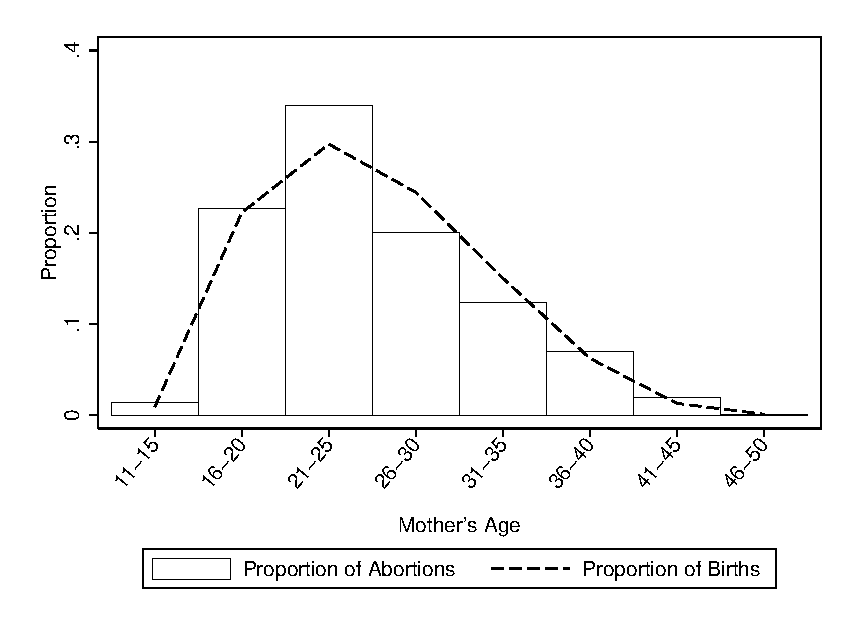
\includegraphics[scale=0.76]{figures/birthDescriptives.eps}
  \caption{Birth and Abortion Descriptives: Mexico}
  \label{MexBirthAbort}
  \vspace{2mm}
  \floatfoot{
    \textsc{Notes to figure}: Total births are plotted between 2002 and 2011.
    Abortions are plotted from the date of reform (April 26, 2007) until 2011.
    The total quantity of births is 23.2 million (all of Mexico), and total
    abortions are 69,861 (Mexico City only).  Births are calculated from
    administrative data (INEGI) and abortions from administrative data (Secretary
    of Health, Mexico DF).}
\end{figure}


\restoregeometry
 
\begin{figure}[H]
\centering	\caption{Trends in Reform and non-Reform Areas}
\label{Trends}
\begin{subfigure}{.5\textwidth}
\centering	\caption{Trends in number of births}\label{birthTrends}
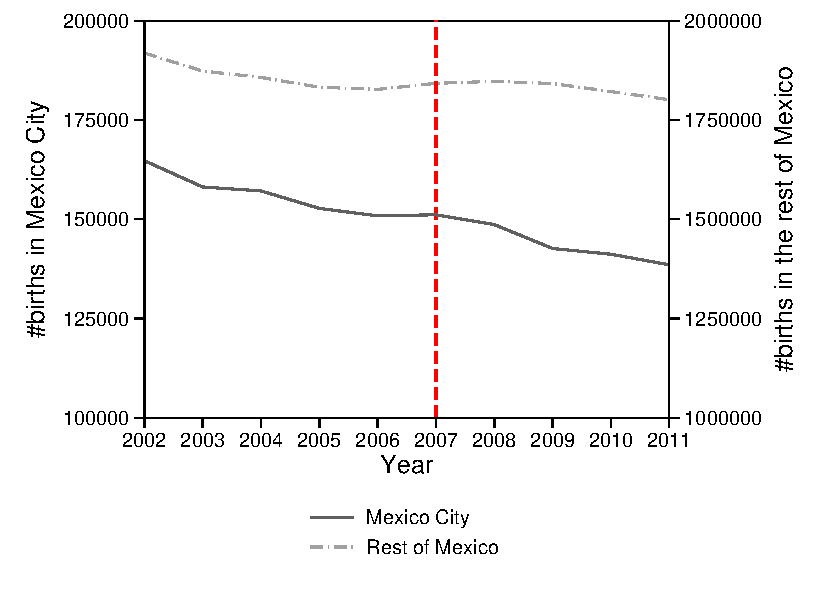
\includegraphics[scale=0.55]{figures/TrendBirth.pdf}
\end{subfigure}%
\begin{subfigure}{.5\textwidth}
\centering\caption{Trends in birth rates}\label{birthrateTrends}
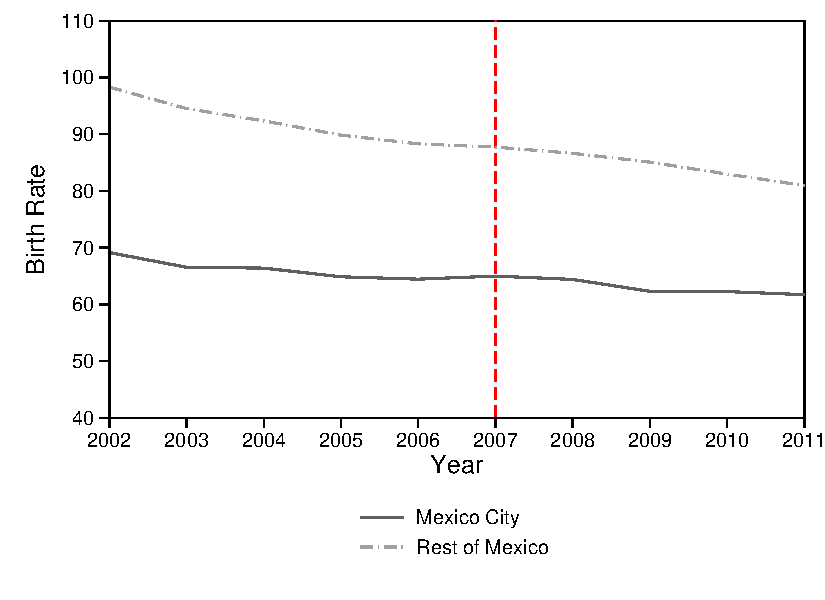
\includegraphics[scale=0.55]{figures/TrendBirthRates.pdf}
\end{subfigure}
\begin{subfigure}{.5\textwidth}
\centering	\caption{Trends in number of maternal deaths}	\label{deathsTrends}
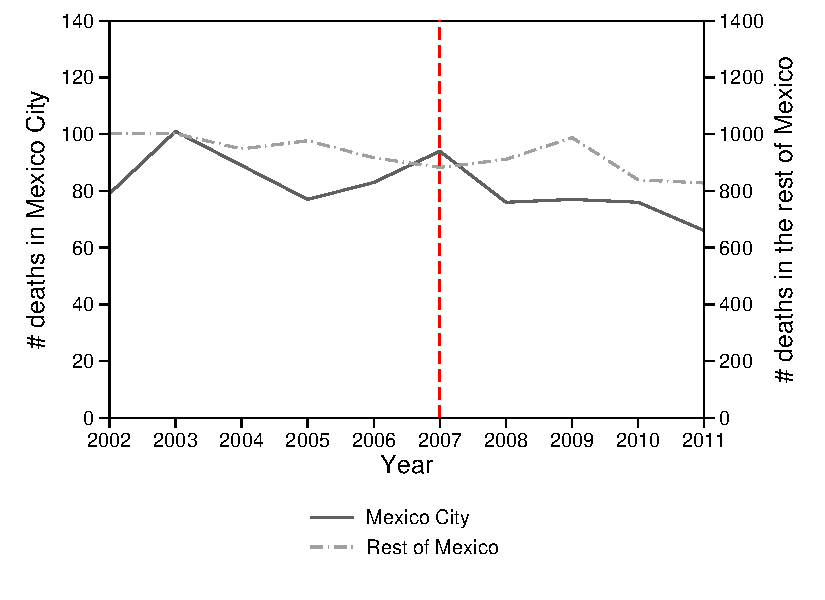
\includegraphics[scale=0.55]{figures/TrendMMR.pdf}
\end{subfigure}%
\begin{subfigure}{.5\textwidth}
\centering \caption{Trends in maternal mortality ratio}	\label{mmrTrends}
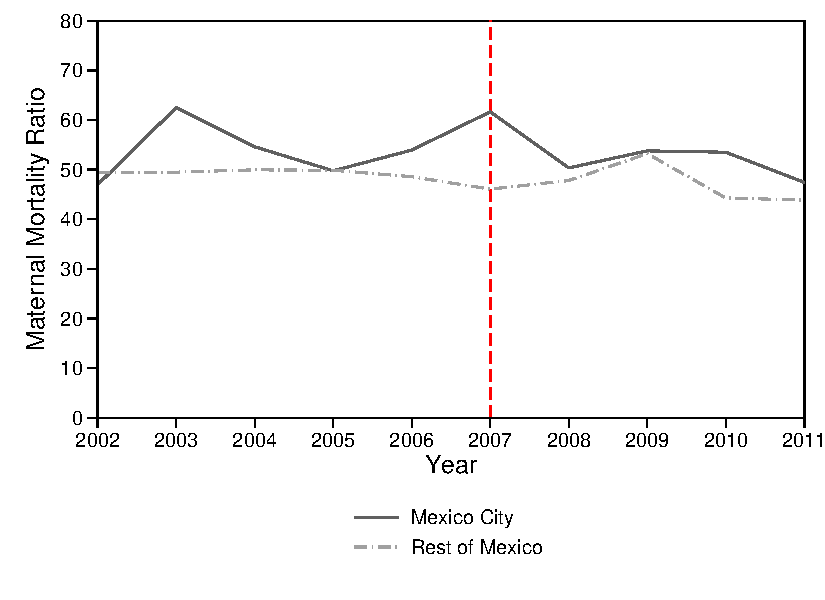
\includegraphics[scale=0.55]{figures/TrendMMratio.pdf}
\end{subfigure} 
\floatfoot{Note to Figure~\ref{Trends}: Each figure is constructed from administrative data made available by INEGI. Trends are constructed based on population weighted means for fertile aged women 15-44. The vertical dashed line indicates the year of the reform. The State of Mexico is excluded due to potential spillover effects. In Figure a) trends in the number of births are displayed. In Figure b) trends in birth rates (the annual number of births per 1,000 women) are presented. In Figure c) the number of maternal deaths are presented followed by the trends in maternal mortality ratio (the annual number of deaths per 100,000 deaths) presented in Figure d). In Figure a) and c) the y-axis to the left shows the levels in Mexico City and y-axis to the right shows the levels in the rest of Mexico.}
 \end{figure}

 
\begin{figure}[H]
\centering	\caption{Placebo tests}
\label{placebo}
\begin{subfigure}{0.5\textwidth}
\centering	\caption{Event study, Fertility}	\label{placebo_birth}
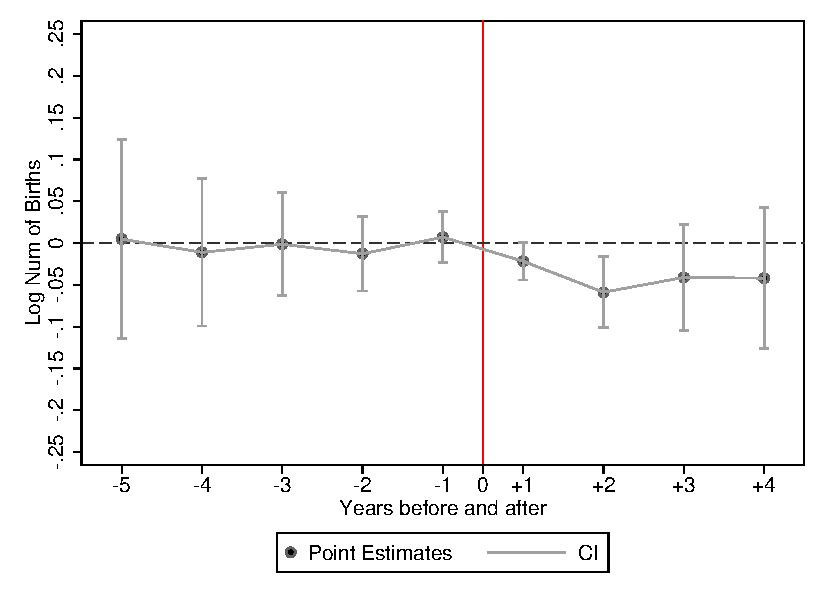
\includegraphics[scale=0.55]{figures/Placeboln_birth.pdf}
\end{subfigure}%
\begin{subfigure}{0.5 \textwidth}
\centering	\caption{Event study, Maternal mortality}	\label{placebo_mmr}
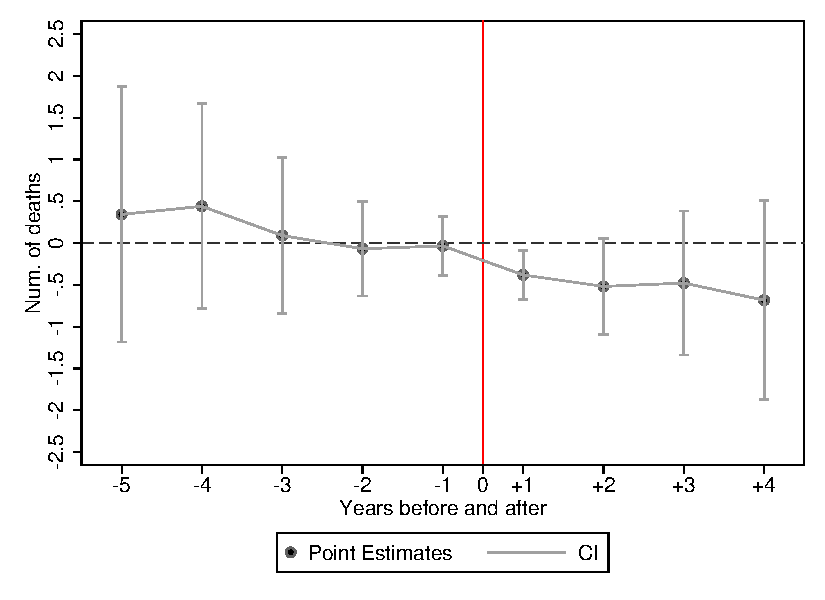
\includegraphics[scale=0.55]{figures/Placebommr.pdf}  	
\end{subfigure}
\floatfoot{Note to Figure~\ref{placebo}: The coefficient plot shows point estimates and confidence intervals estimated using OLS regressions (Figure~\ref*{placebo_birth}) and Poisson regressions (Figure~\ref*{placebo_mmr}). The sample consists of all births and maternal deaths among women aged 15-44 for the period 2002-2011. Leads and lags (5 years before and 4 years after the reform) defined by interaction terms for each year and the treatment area (Mexico City) are included in order to examine anticipatory effects as well as post treatment effects for fertility (a) and maternal mortality (b) respectively. The year of the reform, 2007, is used as the baseline category. The State of Mexico is excluded due to potential spillover effects. A full set of fixed effects, time varying controls and state-specific linear time trends are included in each regression (see note to Table~\ref{MainRegBirth}). }
\end{figure}  



 
\end{spacing}
\end{document}
